\documentclass{isddmaster}
\usepackage[skip=3pt plus1pt]{parskip}
\setlength{\textfloatsep}{12pt plus 2pt minus 4pt}
\setlength{\intextsep}{10pt plus 2pt minus 4pt}
\usepackage{titlesec}
\usepackage{floatrow}
\titlespacing*{\subsection}{0pt}{12pt}{4pt}
\onehalfspacing

\begin{document}
	
	\checkyears
	
	\vspace*{5mm}
	
	\setkeys{Gin}{draft=false}
	
	\selectlanguage{french}   
	
	\def\title{La dynamique de la protease VIH-2 (PR2): \\[5mm] Rapport de Stage M1 }
	\def\candidateaddress{73 rue Albert Dhalenne, 93400 Saint-Ouen-sur-Seine}
	\def\candidatephone{+33767483055}
	\def\labname{BFA CNRS UMR 8251, \\Profilage Pharmacologique In Silico (IsPP)}
	\def\spe{Modélisation des macromolécules} 
	\def\scientificmanager{L. Regad \& M. Baillif}
	\def\labaddress{35 rue Hélène Brion, 75013 Paris}
	\def\author{Anna Perova}
	\def\studentnumber{22519413}
	\def\shorttitle{Rapport de stage}
	\def\mydate{\today}
	\def\keywords{VIH-2, protéase, dynamique moléculaire, état de protonation, distance de Jaccard, arbre de décision}
	
	\pagenumbering{gobble}
	\Entete
	\medskip
	\begin{abstract}
		{\small \textbf{Abstract:} The HIV-2 protease (PR2) is a homodimeric aspartic protease and major therapeutic target whose conformational dynamics govern its catalytic activity. Using the apo crystal structure 1HSI, we conducted four all-atom molecular dynamics simulations ($1000$ ns) under two protonation states of the catalytic dyad Asp25: monoprotonated (MP, V7) and deprotonated (DP, V1, V11, V12). Structural analysis via RMSD, RMSF, inter-residue distances (\text{$d_{50-50}$}, \text{$d_{25-25}$}, \text{$d_{25-50}$}) and a flap projection metric revealed three distinct conformational outcomes. MP systematically stabilizes a classical closed conformation (flap A over flap B) with a rigid catalytic core ($d_{25-25}\approx6,3$\AA). DP induces stochastic behavior: permanent opening (V11), inverted closure with flap B over flap A (V1), or classical closure (V12). Hydrogen bond network analysis demonstrates that classical closure requires a tight interaction cluster around the catalytic site. Hierarchical clustering using pairwise RMSD and Jaccard distance confirms that the closed state of V12 constitutes a structurally distinct alternative to MP closure. These findings provide insights for the rational design of PR2-specific inhibitors.
		
		\textbf{Keywords:} VIH-2, protease, molecular dynamics, protonation state}
		\medskip
		\hrule
		\medskip
		{\small \textbf{Résumé:} La protéase du VIH-2 (PR2) est une protéase aspartique homodimérique et cible thérapeutique majeure dont la dynamique conformationnelle détermine l'activité catalytique. À partir de la structure cristallographique apo 1HSI, quatre simulations de dynamique moléculaire tout-atome ($1000$ ns) ont été réalisées sous deux états de protonation de la dyade catalytique Asp25 : monoprotoné (MP: V7) et déprotoné (DP: V1, V11, V12). L'analyse structurale par RMSD, RMSF, distances inter-résidus (\text{$d_{50-50}$}, \text{$d_{25-25}$}, \text{$d_{25-50}$}) et métrique de projection des \textit{flaps} révèle trois issues conformationnelles distinctes. L'état MP stabilise systématiquement une conformation fermée classique (\textit{flap} A devant \textit{flap} B) avec un cœur catalytique rigide ($d_{25-25}\approx6,3$\AA). L'état DP induit des comportements stochastiques : ouverture permanente (V11), fermeture inversée avec \textit{flap} B devant \textit{flap} A (V1), ou fermeture classique (V12). L'analyse des réseaux de liaisons hydrogène démontre que la fermeture classique requiert l'établissement d'un réseau d'interactions serré autour du site catalytique. La classification hiérarchique par RMSD par paires et distance de Jaccard confirme que l'état fermé de V12 constitue une solution alternative structuralement distincte de la fermeture MP. Ces résultats ouvrent des perspectives pour la conception rationnelle d'inhibiteurs spécifiques à la PR2.
		
		\textbf{Mots clés:} VIH-2, protéase, dynamique moléculaire, état de protonation}
	\end{abstract}
	
	\vfill
	
	\newpage
	\tableofcontents
	\newpage
	
	\pagenumbering{arabic}
	\setcounter{page}{1}
	\section{Introduction}
	
	Le VIH ou virus de l'immunodéficience humaine est un rétrovirus qui conduit au syndrome d'immunodéficience acquise, plus connu comme SIDA. D'après l'Organisation mondiale de la Santé (OMS) et UNAIDS (Programme commun d'Organisation des Nations Unies sur le VIH/SIDA), en 2025, il y avait environ 40,8 millions de personnes atteintes du VIH et environ 630 000 personnes décédées de causes liées au VIH~\cite{noauthor_global_nodate}.
    Même si l'infection par VIH de type 1 (VIH-1) est responsable de la majeure partie de la pandémie mondiale de SIDA, le VIH de type 2 (VIH-2) est une cause importante de maladie dans un certain nombre de régions du monde, surtout en Afrique de l'Ouest~\cite{williams_geographic_2023,van_der_loeff_epidemiology_2008}. De plus, les régions connectées par des liaisons historiques et socio-économiques comme d'autres régions d'Afrique, l'Europe, l'Inde et les États-Unis, observent une augmentation lente et persistante des patients infectés par le VIH-2~\cite{barin_prevalence_2007,soriano_human_2000}. \par
    Les traitements contre l’infection par le VIH-1 ciblent quatre protéines : la protéine de fusion, la protéase (PR), l'intégrase et la transcriptase inverse. Comparée à la thérapie à base d'inhibiteurs non-nucléosidiques de la transcriptase inverse, la thérapie à base d'inhibiteurs de PR a montré un niveau de résistance plus faible~\cite{lv_hiv_2015}.
    Cependant, les inhibiteurs de PR ont toujours de forts effets secondaires, nécessitent un traitement prolongé et produisent des résistances croisées, ce qui encourage les chercheurs à développer de nouvelles approches.
    Pour combattre l'infection par le VIH-2, les mêmes molécules que pour le VIH-1 sont utilisées, telles qu'amprenavir, atazanavir, lopinavir, etc. Malgré 40\% d'homologie au niveau de l'enveloppe et 60\% au niveau des gènes \textit{gag}, il a été démontré que le VIH-2 est naturellement résistant à la plupart de ces inhibiteurs~\cite{desbois_vitro_2008,brower_inhibition_2008,menendez-arias_antiretroviral_2014}.
	Pour ces raisons-là, il est nécessaire d'étudier les spécificités du VIH-2, afin de développer les médicaments adaptés spécifiquement pour le VIH-2.\par
    
	La PR est une protéase \textbf{aspartique}, qui assure le clivage des polyprotéines Gag et Gag-Pol pendant ou juste après la libération du virion de la membrane plasmique, pour produire des protéines matures infectieuses (Annexe \ref{A1}).
    Structurellement, la PR est un homodimère~\cite{chenCrystalStructure19A1994}, composé de deux chaînes polyprotéiques identiques, constituées chacune de 99 acides aminés (Fig.~\ref{fig:PR2_strct}). La protéine peut être découpée en 13 régions structurales et fonctionnelles~\cite{sadiq_explicit_2010}, dont le site actif de la PR qui est formé à l'interface du dimère et contient deux résidus aspartiques catalytiques, chacun étant apporté par l'une des deux sous-unités. Ces résidus appartiennent au motif catalytique, Asp-Thr-Gly (résidus 25 à 27).
    La PR présente également deux feuillets $\beta$, appelés \textit{flaps} qui constituent des régions flexibles, participent à la liaison des substrats et des inhibiteurs~\cite{scott_curling_2000}.
    D'après les données structurales, les \textit{flaps} adoptent différentes conformations, notamment les états semi-ouvert et fermé~\cite{chen_revealing_2014, sadiq_explicit_2010, hornak_hiv-1_2006}. À l'état semi-ouvert (formé sans ligand), les \textit{flaps} sont relevés. Dans cette conformation, le \textit{flap} B est positionné en avant du \textit{flap} A.
    À l'état fermé observé quand la PR est complexée avec un ligand ou un inhibiteur, les \textit{flaps} recouvrent le site actif permettant la stabilisation du ligand.
    Dans cette conformation, le \textit{flap} B est situé en arrière du \textit{flap} A~\cite{baillif_2026_18495249}.\par
    Il est important de comprendre la flexibilité de la protéase de VIH-2 (PR2) et particulièrement les \textit{flaps} en vue de développer des inhibiteurs spécifiques pour la PR2.
	Cong et al. en 2018 ont montré que l'état de protonation du résidu catalytique Asp25 de la chaine B impactait la dynamique de la PR2 \cite{congExploringReasonsDecrease2018}.  
    Cependant l'impact de la protonation du site actif sur la conformation de la protéase et sa flexibilité n'a jamais été étudié en détail.\par
    Pour répondre à cette question, plusieurs simulations de dynamique moléculaire (DM) de PR2 dans sa forme apo (semi-ouverte) ont été réalisées dans l'état de monoprotonation (MP) et de déprotonation (DP) du site catalytique.

	L'objectif de ce stage consiste en l'analyse et la comparaison des simulations de dynamiques moléculaires afin de définir l'impact de l'état de monoprotonation du site catalytique (Asp25, chaîne B) sur la conformation protéique, ainsi que sur la flexibilité globale et locale de la PR2.
	\begin{figure}[hb!]
		\centering
		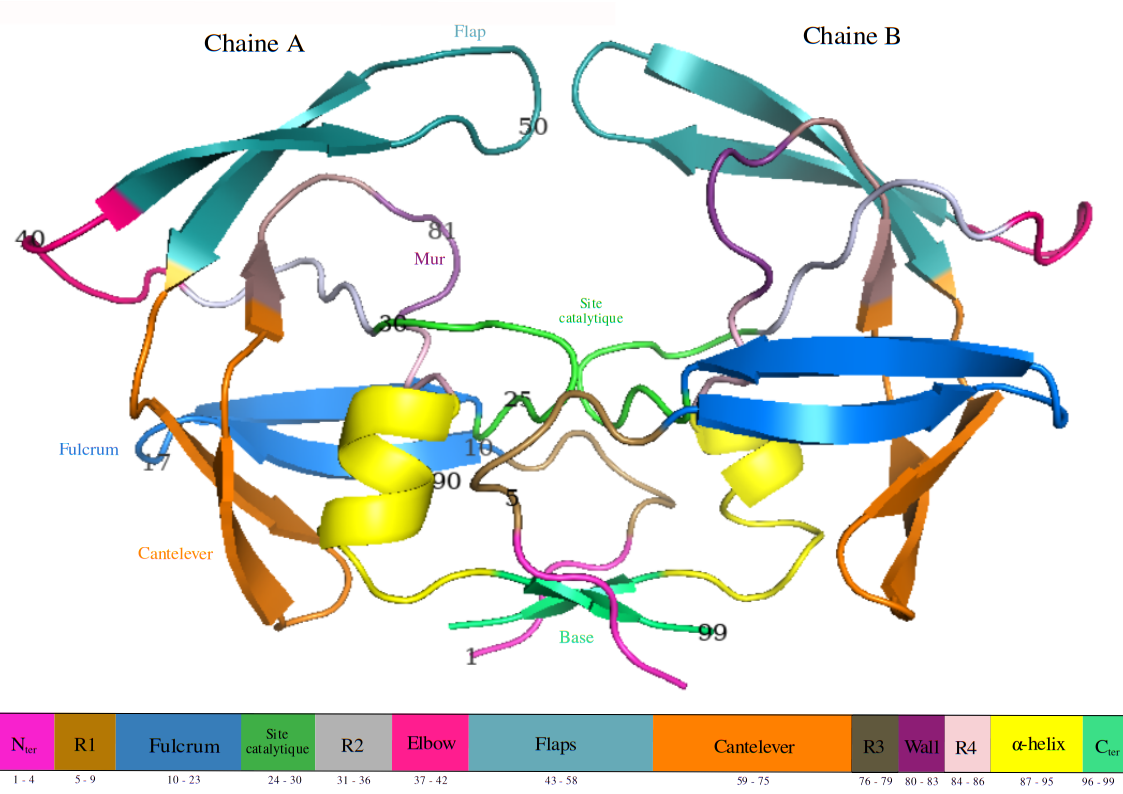
\includegraphics[width=0.75\linewidth]{Figures/PR2_structure_1.png}
		\caption{La structure tridimensionnelle de la protéase dimère VIH-2. Structure à partir d'entrée PDB 1HSI.}
		\label{fig:PR2_strct}
	\end{figure}

	
	\section{Matériels \& Méthodes}
	\subsection{Simulations de Dynamique Moléculaire}
		\begin{wraptable}[9]{r}{0.5\textwidth}
		\vspace{-10pt}
			\centering
		\begin{tabular}{@{}lll@{}}
			\toprule
			\textbf{Condition} & \textbf{Nom}  & \textbf{Tps de sim (ns)}  \\ \midrule
			Déprototoné (DP)   & V11          & 1 000       \\
			Déprototoné (DP)   & V12          & 1 000       \\
			Déprototoné (DP)   & V1           & 1 000       \\
			Monoprotoné (MP)   & V7           & 1 000               
		\end{tabular}
		\caption{Tableau récapitulant les 6 simulations étudiées et ses conditions}
		\label{tab:simulations}
	\end{wraptable}
	Les simulations de DM ont été réalisées en utilisant la structure cristallographique de PDB 1HSI (résolution de 1.9 \AA), seule structure en forme non complexée (apo) de PR2 disponible dans la base de données PDB.
    Quatre simulations ont été lancées à partir de cette structure en utilisant différentes conditions de simulations : 1 en conditions déprotonées ou DP : V7 et 3 en conditions monoprotonées ou MP : V1, V11, V12 (Table~\ref{tab:simulations}).
    L'hydrogène rajouté pour les DM en conditions MP se trouve au niveau de carbone-$\delta$ d'Aspartate 25 de la chaine B (Fig.~\ref{fig:protonation}).
    Les simulations de DM ont été réalisées pendant 1000 ns, en conditions de solvant explicite et en considérant tout atome (\textit{AAMD}).
    Les conditions de MP ont été démontrées reproductibles grâce aux deux simulations réplicats V8 et V21, qui ont démontré des résultats similaires pour les métriques analysées dans ce rapport.
    \begin{figure}[h]
		\centering
		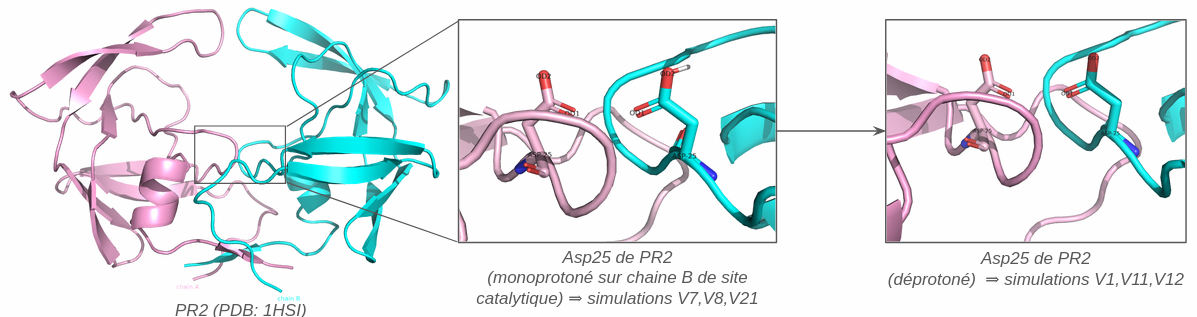
\includegraphics[width=0.85\linewidth]{Figures/protonation_on_1HSI.png}
		\caption{Visualisation de la structure monoprotonée (utilisée pour V7,V8,V21) et déprotonée (utilisée pour V1,V11, V12).}
		\label{fig:protonation}        
	\end{figure}
	
	Les simulations de DM ont été effectuées hors de ce stage et le protocole peut être retrouvé en annexes (\ref{A2}). Les résultats des simulations ont été analysés visuellement avec VMD~\cite{HUMP96} et PyMol~\cite{PyMOL}, ainsi que numériquement en Python (packages \lstinline{MDAnalysis}~\cite{gowersMDAnalysisPythonPackage2016},\cite{michaud-agrawalMDAnalysisToolkitAnalysis2011} et \lstinline{MDtraj}~\cite{McGibbon2015MDTraj}) et R (package  \lstinline{bio3D}~\cite{grantBio3dBiologicalStructure2024}). Les codes développés pendant ce stage sont tous accessibles sur \href{https://github.com/annhater/M1_STAGE}{GitHub}.

	\subsection{Métriques d'Analyse Structurale}
	\subsubsection{$\text{RMSD}_{\text{stepwise}}$}
	Afin d'évaluer l'impact de la protonation sur la stabilité du système, nous avons comparé la stabilité du système au cours de différentes simulations en calculant le \textit{Root Mean Square Deviation} (RMSD). Le RMSD (Annexe~\ref{A3}) mesure la distance entre la conformation de la protéine au moment $x$ (frame $x$) contre la structure de départ (frame 0).
	Pour les valeurs de RMSD, les carbones $\alpha$ de chaque frame de simulation ont été alignés sur les carbones $\alpha$ de la structure de départ.
	
	\subsubsection{RMSF}
	Pour localiser les régions qui se déforment au cours de la simulation, nous avons calculé le \textit{Root Mean Square Fluctuation} (RMSF) des carbones $\alpha$ (C$_\alpha$) de chaque résidu de PR2. Le RMSF (Annexe \ref{A4}).
	Lorsqu'on a défini comment la structure évolue au cours du temps, on voudrait préciser quels sont les résidus qui sont impliqués dans le changement conformationnel mesurant l'écart de la position d'une particule (dans notre cas les C$_\alpha$) par rapport à une position de référence (position d'atome moyenne) dans le temps.
	\subsubsection{Distances inter-résidus}
	Afin de caractériser plus finement les déformations au cours de simulations, nous avons calculé les distances entre les C$_\alpha$ de certains résidus d’intérêt.
    Les distances $d_{50-50}$, $d_{25-25}$, $d_{25-50}$ ont été calculées.
    Afin de caractériser plus finement les déformations au cours des simulations, nous avons calculé les distances entre les $\text{C}_\alpha$ de certains résidus clés du site catalytique et des \textit{flaps}.
    Plus précisément, les distances inter-résidus $d_{50-50}$, $d_{25-25}$ et $d_{25-50}$ ont été suivies tout au long des trajectoires de DM. La distance $d_{50-50}$ sert d'indicateur direct du degré d'ouverture ou de fermeture des \textit{flaps}, qui démontre l'accessibilité du site actif.
    La distance $d_{25-25}$ permet quant à elle d'observer la stabilité structurale de la dyade catalytique dépendant de l'état de protonation.
    Enfin, les distances $d_{25-50}$ caractérisent le rapprochement vertical des \textit{flaps} vers le cœur de la protéase, nous permettant ainsi de détecter d'éventuels comportements asymétriques entre les chaînes A et B. 
    
	\subsubsection{Projection de résidu 50 de la chaîne B sur le plan défini par les résidus 49, 50, et 51 de la chaîne A}
	Pour caractériser l'orientation des \textit{flaps} entre eux lors de la simulation, nous avons calculé la métrique de projection de résidu 50 de la chaîne B sur le plan défini par les résidus 49, 50, et 51 de la chaîne A ($d_{50B\xrightarrow{}49-50A-51A}$).
    Cette métrique développée par mes encadrantes~\cite{baillif_2026_18495249}, permet de caractériser la position du \textit{flap} B par rapport au \textit{flap} A (le long de la perpendiculaire au plan du \textit{flap}).
    La valeur négative de cette métrique indique que le \textit{flap} A se trouve devant le \textit{flap} B, la conformation qui est observée dans les conformations fermées dans la littérature. La valeur positive indique que le \textit{flap} B, se trouve devant le \textit{flap} A. Cela est notamment retrouvé dans le cas de la conformation semi-ouverte que nous appelons "inverse" par la suite.

	\subsubsection{Classification des structures extraites de V7 et V12}
	Afin de déterminer si les mécanismes de fermeture des trajectoires V7 et V12 reposent sur des bases structurales identiques, nous avons mis en place une approche de classification comparative s'appuyant sur deux échelles d'analyse : la géométrie globale du squelette peptidique et le réseau dynamique des interactions locales.
    Dans un premier temps, la similarité de la conformation globale a été évaluée par le calcul du $\text{RMSD}_{\text{pairs}}$. Contrairement au $\text{RMSD}_{\text{stepwise}}$ qui suit l'évolution temporelle d'une unique trajectoire, cette métrique calcule la distance atomique entre chaque structure (\textit{frame}) de la simulation V12 et chaque structure de la simulation V7, cette dernière étant établie comme notre référence en conditions de protonation de type monoprotoné (MP). Ce calcul permet de générer une matrice carrée de distances inter-trajectoires (Annexe \ref{A5}), mettant en évidence les similitudes et les divergences des mouvements atomiques par paires de configurations.
    Dans un second temps, pour capturer la réorganisation fine des interactions au cours de la fermeture, nous avons analysé l'évolution du réseau de liaisons hydrogène. La similarité de ces profils d'interactions entre les deux simulations a été quantifiée par la distance de Jaccard, qui mesure le degré de similitude entre deux ensembles d'objets (Eq. \ref{eq:jaccard}), où 0 représente une absence totale de similarité et 1 représente une similarité parfaite. Ici, les objets comparés correspondent à la présence ou l'absence des liaisons hydrogènes spécifiques au sein de chaque structure.
	\begin{equation}{}
		{\displaystyle J(A,B)={\frac {|A\cap B|}{|A\cup B|}}={\frac {|A\cap B|}{|A|+|B|-|A\cap B|}}}
		\label{eq:jaccard}
	\end{equation}

	Ces deux métriques de distance ($\text{RMSD}_{\text{pairs}}$ et Jaccard) ont ensuite été exploitées via des méthodes d'analyse multivariée pour classifier l'ensemble des structures. Nous avons d'une part réalisé une classification ascendante hiérarchique (CAH) utilisant le critère d'agrégation de Ward. Ce choix méthodologique permet de minimiser la variance intra-classe afin de regrouper les \textit{frames} de V7 et V12 au sein d'un dendrogramme selon leur proximité géométrique ou d'interaction, révélant ainsi d'éventuels états conformationnels partagés.
	\section{Résultats}
	Pour répondre à la question --~\emph{Quel est l'impact de la protonation sur le comportement dynamique de la PR2?} -- nous avons analysé les DM de la PR2 sous forme apo sous différentes conditions de protonation.
	
	\subsection{Étude de la stabilité de la PR2 selon l'état de protonation}
	Dans un premier temps, on a étudié l'impact de la protonation sur la stabilité du système en calculant le $\text{RMSD}_{\text{stepwise}}$ par les pas de la simulation (Fig.~\ref{fig:RMSD}).
    Comparé à la simulation MP (V7), les valeurs de $\text{RMSD}_{\text{stepwise}}$ varient beaucoup plus pour les simulations déprotonées: V1 et V11. Pour V11, la phase de stabilisation est absente. Pour V1, la stabilisation est observée vers 
    L'analyse de la dynamique globale de la protéine au cours de la simulation nous a permis d'observer les changements conformationnels qui se produisent au cours de la simulation.
    Les valeurs de la métrique $\text{RMSD}_{\text{stepwise}}$ nous ont permis d'observer les différences globales qui se produisent au cours de la simulation et les différences entre les deux conditions de protonation.
	Pour toutes les simulations, sauf V11, nous observons une stabilisation des valeurs $\text{RMSD}_{\text{stepwise}}$. Pour V7 (MP) la stabilisation est obtenue vers $2$~\AA. Pour les DP,  nous observons trois cas différents : V12, qui se stabilise vers $2,5$~\AA, V1, qui se stabilise vers $3,5$~\AA, et V11, qui ne se stabilise pas et augmente jusqu'à $6$~\AA.\par 

	\begin{figure}[h]
        \centering
        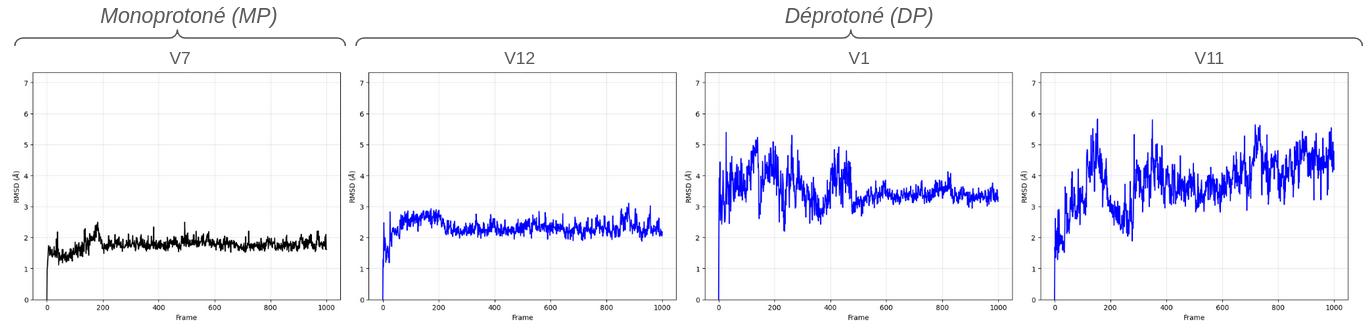
\includegraphics[width=\linewidth]{Figures/RMSD_new.png}
        \caption{Analyse de $\text{RMSD}_{\text{stepwise}}$ (fluctuation moyenne quadratique de chaque frame par rapport à la structure initiale) entre les quatre simulations étudiées : DP (V1,V11,V12) en bleu contre référence MP (V7) en noir. RMSD calculé sur les C$_\alpha$.}
        \label{fig:RMSD}
    \end{figure}

    \subsection{Étude de flexibilité de la PR2 selon l'état de protonation} \label{sec:RMSF}
    Par la suite, nous avons exploré plus précisément l'impact de la protonation sur la flexibilité de la structure et quels sont les résidus les plus mobiles au cours des simulations.
    Pour cela, nous avons fait une analyse de RMSF, qui permet d'accéder aux variances des positions atomiques au cours de la simulation (Fig.~\ref{fig:RMSF}).
    Nos résultats ont démontré des pics de flexibilité autour des résidus 50 et 149 (\textit{flaps}), pour toutes les simulations, ce qui est en accord avec la littérature, qui insiste sur l'importance des \textit{flaps} dans la conformation finale. 
    Pour les V1 et V11 nous observons des pics de flexibilité autour des résidus 25-30 (site catalytique), ainsi que des pics plus prononcés autour des résidus 50-51 (\textit{flaps}).
    Pour la simulation V12 (DP), nous observons une ressemblance de profil à la simulation MP, avec des \textit{flaps} toujours flexibles, mais beaucoup plus rigides comparés à V1 et V11.
	
	\begin{figure}[h]
        \centering
        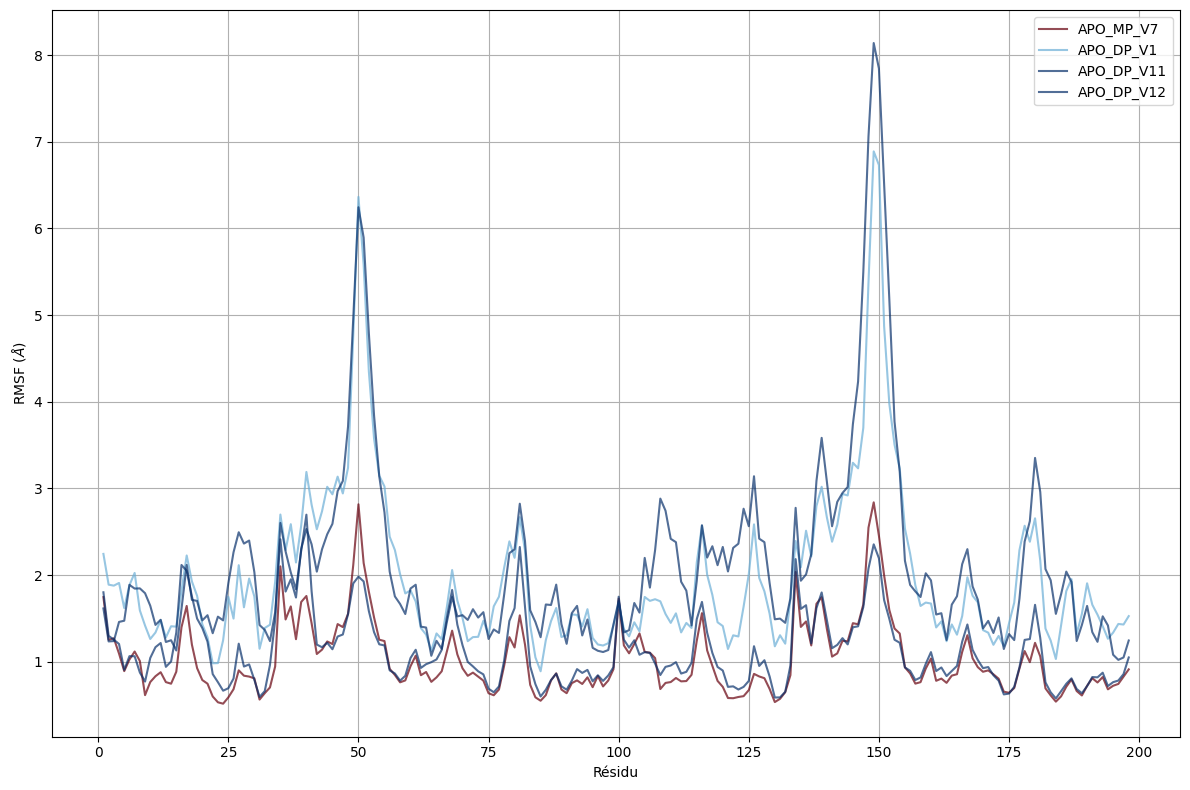
\includegraphics[width=0.6\linewidth]{Figures/rmsf_new.png}
        \caption{Analyse RMSF (fluctuation moyenne quadratique) entre les quatre simulations étudiées: DP (V1,V11,V12) en nuances de bleu contre la référence MP (V7) en rouge. RMSF calculé sur les C$_\alpha$ après un ajustement sur le squelette protéique.}
        \label{fig:RMSF}
    \end{figure}

    \subsection{Étude de la conformation des \textit{flaps} selon l'état de protonation}
    Les résultats d'étude de la dynamique globale et de flexibilité nous ont permis de définir les régions d'intérêt pour l'analyse plus détaillée, qui sont : les résidus 50-51 (\textit{flaps}) et les résidus 25-30 (site catalytique).
    Cela nous a amené à continuer vers l'analyse de variation des distances entre les résidus d'intérêt.
    

    La distance $d_{50-50}$ explique la dynamique d'ouverture et de fermeture des \textit{flaps} (Fig.~\ref{fig:d50}). Dans la simulation V7 (MP) et le réplicat V12 (DP), la convergence vers une valeur stable de $d_{50-50} \approx 7,3$~\AA~confirme la stabilisation vers la forme fermée.
    Pour le système V1, la distance se stabilise à une valeur plus élevée ($13,0$~\AA), reflétant une conformation plus ouverte. Enfin, la trajectoire V11 montre des fluctuations majeures atteignant $43$~\AA, indiquant sur la forme toujours ouverte.
    On fait des conclusions similaires en analysant les distances $d_{25-50}$ (Annexe \ref{A6}), qui montrent que les \textit{flaps} se rapprochent du cœur de la protéase dans V7 et V12, tandis que pour V1 et V11, les \textit{flaps} restent éloignés du cœur, ce qui peut expliquer l'incapacité de ces systèmes à maintenir une conformation stable et fermée avec \textit{flap} B derrière \textit{flap} A.


    \begin{figure}[h]
        \centering
        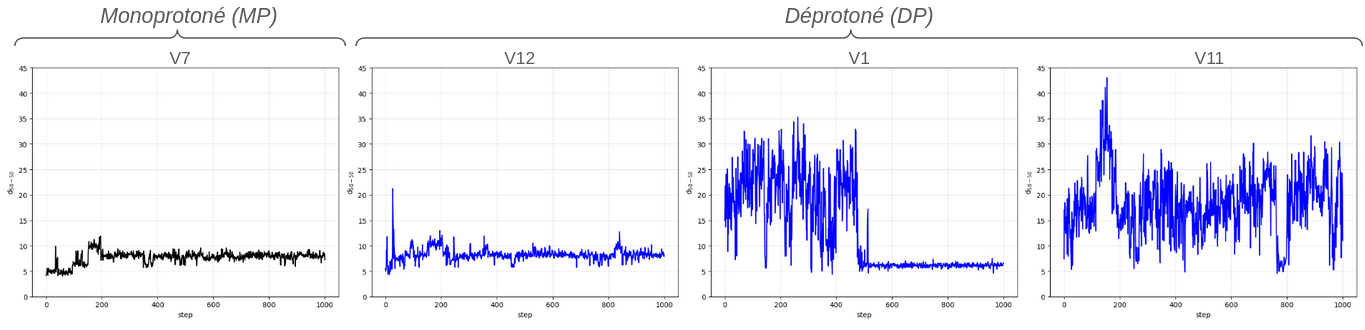
\includegraphics[width=\linewidth]{Figures/d_50_new.png}
        \caption{Analyse $d_{50-50}$ entre les dimères pour les quatre simulations : DP (V1,V11,V12) en bleu contre la référence MP (V7) en noir.}
        \label{fig:d50}
    \end{figure}

Afin d'approfondir notre compréhension de la dynamique conformationnelle des \textit{flaps}, nous avons appliqué une métrique de projection tridimensionnelle, notée $d_{50B\xrightarrow{}49-50A-51A}$ (Fig.~\ref{fig:d50_projection}).
Ce descripteur géométrique permet de suivre précisément la position relative des deux \textit{flaps} l'un par rapport à l'autre au cours du temps.
L'analyse des trajectoires à travers cette métrique révèle trois profils de distances distincts. Un profil stable et négatif est observé pour la simulation V7 (MP) et le réplicat V12 (DP). Après une brève phase initiale de fluctuation avec les valeurs positives, ces trajectoires convergent et se stabilisent vers des valeurs négatives (autour de $-4$ à $-5$~\AA).
Un profil stable et positif caractérise la simulation déprotonée V1. Lors de sa transition vers la stabilisation (à partir de 517~ns), la valeur de projection se stabilise dans des valeurs positives (autour de $+3$~\AA).
Un profil de fortes fluctuations est visible pour le réplicat déprotoné V11, où la valeur de projection oscille de manière erratique sans jamais se stabiliser, oscillant entre des valeurs positives et négatives.
Sur le plan structural, ces différents profils se traduisent par des arrangements spatiaux très spécifiques des \textit{flaps}. Les valeurs négatives (V7 et V12) signifient que la PR2 adopte et maintient une fermeture dite "classique", où le \textit{flap} A vient se positionner physiquement au-dessus du \textit{flap} B.
Il a été démontré que ces conformations sont proches des structures de la PR2 co-cristallisées avec les ligands.
À l'inverse, les valeurs positives dans les structures de V1 caractérisent le fait que dans ces structures nous observons le \textit{flap} B qui reste devant le \textit{flap} A, stabilisant la PR2 dans une conformation fermée mais avec des \textit{flap} inversés.
Enfin, les fluctuations majeures de V11 confirment que les \textit{flaps} restent incapables de s'apparier, ce qui correspond à l'état continuellement ouvert identifié précédemment.
\par
Nous pouvons suggérer que pour la fermeture de \textit{flaps}, le rearrangement de \textit{flaps} n'est pas nécessaire.
Par contre, pour atteindre une conformation stable au niveau du site catalytique (comme nous avons vu en section \ref{sec:RMSF}), la fermeture de \textit{flaps} correcte (A devant B) est indispensable.

    \begin{figure}
        \centering
        \vspace{-10pt}
        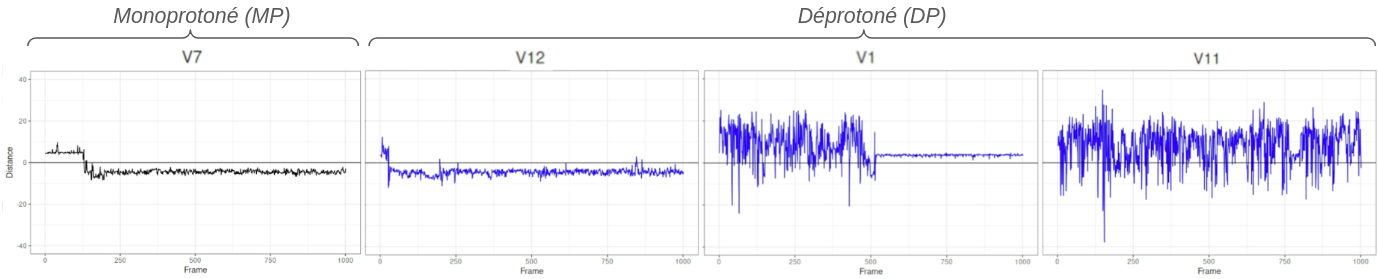
\includegraphics[width=\linewidth]{Figures/d50_projection_new_line.png}
        \caption{Analyse de la projection $d_{50B\xrightarrow{}49-50A-51A}$ pour les quatre simulations : DP (V1,V11,V12) en bleu contre référence MP (V7) en noir. Une valeur de projection négative indique que le \textit{flap} A est devant le \textit{flap} B, alors qu'une valeur positive indique l'inversion des \textit{flaps}.}
        \label{fig:d50_projection}
    \end{figure}
    



    \subsection{Étude de la conformation du site catalytique selon l'état de protonation}
    \begin{wrapfigure}[19]{r}{0.65\textwidth}
        \centering
        %\vspace{-15pt}
        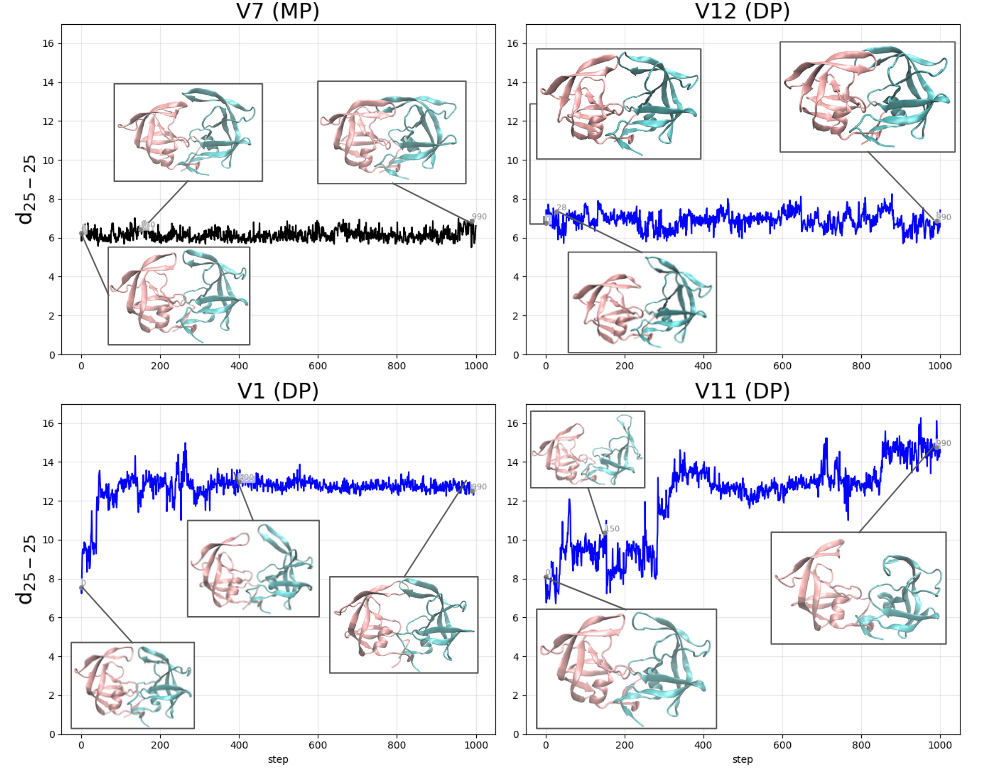
\includegraphics[width=\linewidth]{Figures/d_25_25_w_frames.png}
        \caption{Analyse $d_{25-25}$ entre les dimères pour les quatre simulations : DP (V1,V11,V12) en bleu contre référence MP (V7) en noir. Les snaphots ont été rajoutés pour illustrer l’évolution de la structure au cours de la simulation.}
        \label{fig:d25_25}
    \end{wrapfigure}

    L'analyse de la distance $d_{25-25}$ (Fig.~\ref{fig:d25_25}) qui caractérise la géométrie du site catalytique révèle toujours une forte hétérogénéité pour les trajectoires déprotonées: V1 et V11. 
    Le réplicat avec fermeture des \textit{flaps} inversé V1 montre quant à lui une stabilisation intermédiaire autour de $12,6$~\AA. 
    En revanche, pour le réplicat ouvert V11, la distance $d_{25-25}$ oscille au cours de la simulation et atteint un maximum de $16,3$~\AA, ce qui indique une déformation irréversible et un écartement du cœur de la protéase. Au contraire, le réplicat V12 (fermeture classique) maintient la distance entre les deux C$_\alpha$ des Asp25 stable à $6,9$~\AA, comparable au système MP avec la valeur moyenne de $6,3$~\AA.
    Ce maintien rigide confirme que la monoprotonation verrouille la géométrie fonctionnelle du site catalytique.

    \begin{wrapfigure}[24]{r}{0.4\textwidth}
        \centering
        \vspace{-18pt}
        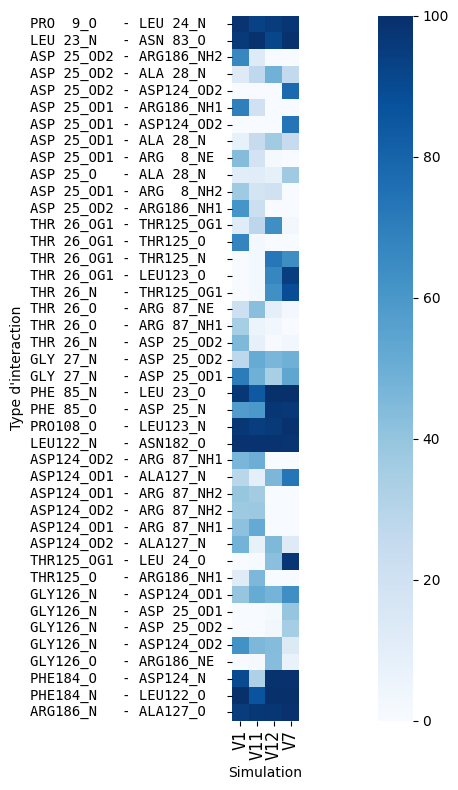
\includegraphics[width=\linewidth]{Figures/interactions_heatmap_new.png}
        \caption{Heatmap de fréquences d'apparition de liaisons hydrogènes impliquant les résidus du site catalytique : résidus 23-27 de chaine A (1 à 99) et chaine B (100 à 198) au cours de la simulation.\\
Notation : \lstinline{RESNAME_RESNUM_ATOM 1 - RESNAME_RESNUM_ATOM 2}.} 
        \label{fig:interaction_heatmap}
    \end{wrapfigure}
    Comme nous avons identifié que la protonation agit sur le mouvement des \textit{flaps} et la stabilisation du site catalytique, il était dans notre intérêt d'analyser plus en détail les interactions qui se forment autour du site catalytique. Nous supposons qu'il pourrait y avoir une corrélation entre la formation des liaisons stabilisantes et la stabilisation du système avec un arrangement des \textit{flaps} correct.
    En analysant les interactions intra-protéiques (liaisons hydrogènes) impliquant les résidus du site catalytique (Fig.~\ref{fig:interaction_heatmap}), nous notons la différence évidente entre la simulation MP et les réplicats DP : l'absence d'interaction de dyade catalytique (\lstinline{ASP 25_OD1/ASP 25_OD2 - ASP 124_OD2}). Par la suite, nous observons la presence plus fréquente des interactions du site catalytique avec Arg8 de R1 (\lstinline{ASP 25_OD1 - ASP 8_NE}) et Arg87 d’hélice $\alpha$ (\lstinline{ASP 26_O - ASP 87_NE/ASP 87_NH1, ASP 25_OD2 - ARG186_NH1}) pour les V1 et V11.
    Nos analyses précédentes ont montré que la PR2 de la simulation V12 a le même comportement que la PR2 de la simulation V7.
    Sur la Fig.~\ref{fig:interaction_heatmap} nous remarquons que ces deux simulations présentent une conservation des interactions (\lstinline{THR 26_OG1 - THR 125_N, THR 26_OG1 - LEU 123_O, THR 26_N - THR 125_OG1, THR 25_OG1 - LEU 24_O}). Ce résultat suggère que ces interactions pourraient être responsables de la stabilisation du site actif.
    
    \par En regardant les liaisons hydrogènes autour du site catalytique (Fig.\ref{fig:coeur_prot}), nous notons des différences en conformation du cœur protéique en fonction de la simulation. Pour la simulation V11, les résidus du cœur protéique (8, 25-27 et 97) sont éloignés et ne rentrent pas en contact.
    Pour la simulation V1, nous observons ces résidus en se rapprochant, avec les résidus du site catalytique en rentrant en interaction, mais sans implication du résidu 9 du R1.

    Pour les deux V12 (DP) et V7 (MP), nous observons la formation d'un réseau d'interactions serré et peu flexible autour du site catalytique, qui ressemble à un bouchon.
    
    Ces résultats suggèrent un lien entre la stabilité du site catalytique et la fermeture des \textit{flaps}.
    L'absence de protonation se répercute sur la capacité de former des liaisons stabilisantes au niveau du site catalytique. Possiblement, pour cette raison, l'apparition des \textit{flaps} de façon symétrique et fonctionnelle est un événement plus rare (uni V12).
	
	\begin{figure}[h]
        \centering
        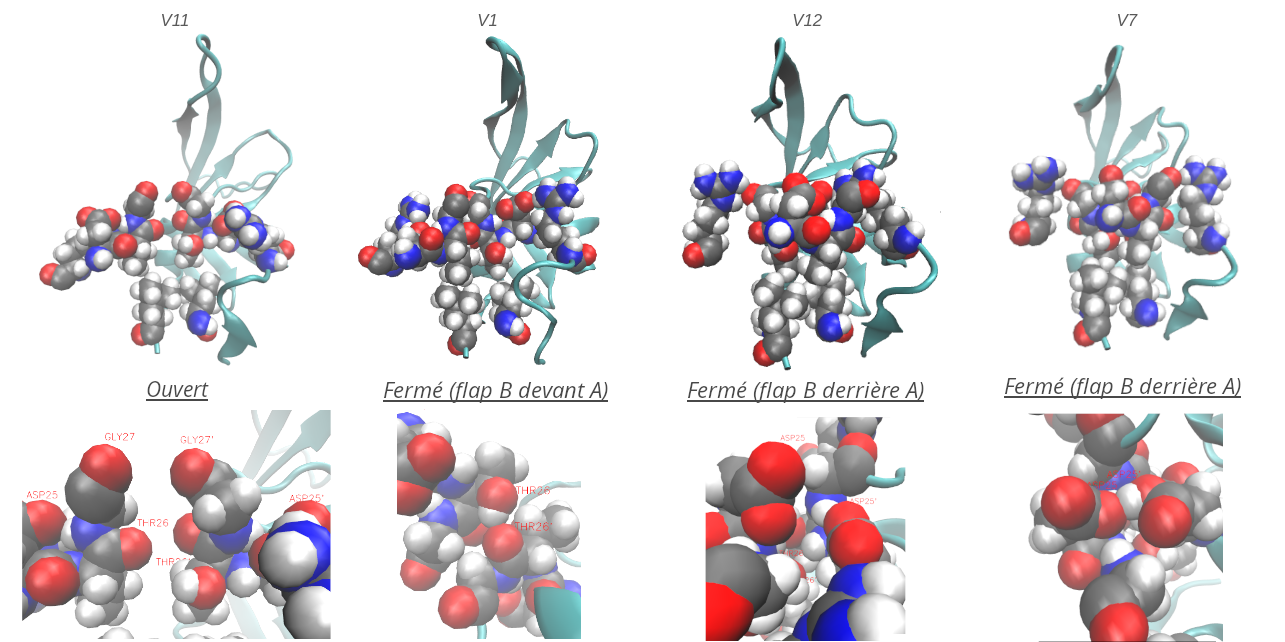
\includegraphics[width=\linewidth]{Figures/coeur_prot_new.png}
        \caption{Visualisation du cœur protéique (résidus 8, 25-27 et 97 de deux chaînes) en VMD pour les simulations V7, V12, V1 et V11. Snapshot pris à la fin de la simulation (frame 1000). Une partie de la chaine A a été omise pour meilleure visibilité.}

        \label{fig:coeur_prot}
    \end{figure}
    
    \subsection{Classification hiérarchique de structures de V7 et V12}
    Tout au long de notre étude, nous avons mis en évidence que le réplicat DP V12 adopte un comportement qui ressemble fortement à celui des structures MP, aboutissant à une conformation fermée classique. Afin d'explorer si ces deux formes finales sont identiques sur le plan géométrique et de leurs réseaux d'interactions, nous avons implémenté une approche de classification hiérarchique. Pour ce faire, nous avons séparé les trajectoires de V7 (MP) et V12 (DP) en deux périodes distinctes : la Phase 1 ($\phi_1$), représentant l'état initial fluctuant avant le basculement des \textit{flaps}, et la Phase 2 ($\phi_2$), correspondant à l'état final fermé et stabilisé.\par
    Dans un premier temps, nous avons évalué la proximité géométrique globale des structures par le calcul d'une matrice de $\text{RMSD}_{\text{pairs}}$, restituée sous forme de dendrogramme (Annexe \ref{A7}). Les résultats montrent une séparation qui isole d'un côté l'ensemble des structures de la $\phi_1$, et de l'autre les structures de la $\phi_2$. Toutefois, au sein de ce groupe de $\phi_2$, les formes fermées finales de V7 et V12 sont séparées par simulation et présentent une longue distance entre elles. L'absence de mélange entre les deux trajectoires indique que, malgré une apparence similaire, les mouvements internes de la forme fermée de V12 diffèrent de ceux de la forme fermée classique de V7.\par
    Dans un second temps, nous avons cherché à comprendre l'origine moléculaire de cette divergence géométrique finale. Notre hypothèse étant que les réarrangements locaux lors du basculement des \textit{flaps} dictent la conformation de l'état final, nous avons focalisé notre analyse des liaisons hydrogène autour de la fenêtre de transition ($\pm36$ ns).
    
	Le suivi des interactions au moment précis de ce basculement, quantifié par la distance de Jaccard, permet de capturer l'établissement des contacts critiques qui guident le système vers son puits de potentiel final.
    Le dendrogramme des interactions (Annexe \ref{A7}) révèle que si la phase $\phi_1$ de V7 s'isole, un unique grand cluster regroupe à la fois la phase $\phi_2$ de V7 et l'intégralité des deux phases de V12.
    Ces observations nous conduisent à une conclusion que d'une part, la monoprotonation dans V7 induit la mise en place d'interactions uniques et spécifiques en $\phi_2$ qui ne peuvent pas apparaître en conditions DP, ce sont ces contacts qui possiblement stabilisent la forme fermée et stable de la PR2 avec les \textit{flap} B derrière \textit{flap}.
    D'autre part, dans le cas DP, les interactions requises pour stabiliser une forme fermée sont plus rares (uniquement en V12), mais possibles. La forme fermée obtenue en $\phi_2$ de V12 n'est pas égale à la forme classique de MP, mais constitue une solution alternative.
    Cette conformation alternative compense l'absence de proton en établissant un réseau d'interactions qui joue le même rôle de stabilisation du cœur enzymatique.

	\section{Discussion \& Conclusions}
    Au cours de ce projet de stage, nous nous sommes focalisés sur l'exploration des événements qui sont à la base de la fermeture de la structure de la protéase PR2 (1HSI). Les DM réalisées en deux conditions -- monoprotoné et déprotoné -- nous ont révélé trois types de structure finale possible : ouverte (V11), fermée avec le sens des \textit{flap} A devant B et cœur protéique stable (V7,V12) et fermée mais avec \textit{flap} B devant A et cœur protéique flexible (V1).
    Nous avons pu conclure que la monoprotonation stabilise toujours le système et cause la fermeture avec \textit{flap} A devant \textit{flap} B. Au contraire, la déprotonation cause 3 comportements. Le premier comportement est proche de celui observé en MP, correspondant à une PR2 qui soulève les \textit{flaps} pour que le \textit{flap} B se pose derrière le \textit{flap} A et se referme, si le système peut se stabiliser au cours de la simulation (V12). Sinon, le système reste très flexible au cours de la simulation (V1, V11).
    Grâce aux analyses d'environnement autour du site catalytique, nous avons pu identifier des interactions qui jouent un rôle dans la stabilisation de la structure en conditions déprotonées, que la structure en V12 a réussi à former.
    \par En perspective, nous pourrions analyser plus précisément les interactions qui différencient les formes fermées de V7 et V12, ainsi qu'analyser l'espace 3D du site catalytique plus en détail, pour mettre en évidence le rôle d'un réseau d'interactions dans la fermeture.
    %De plus, on vise à construire une carte d'interactions à ce niveau-là, pour voir si d'autres événements peuvent jouer un rôle dans la stabilisation de la structure fermée.
    Cette étude pourrait être potentiellement utile dans la conception d'inhibiteurs spécifiques au VIH-2, en soulignant que même dans des conditions DP, la PR2 parvient à se stabiliser et à se fermer.
	
	\section{Remerciements}
	Ce stage de master a été effectué au sein de l'équipe Profilage Pharmacologique In Silico (IsPP) de l'unité de Biologie Fonctionnelle et Adaptative (BFA) de l'Université Paris Cité, sous la direction de \textbf{Dr. Leslie Regad} et de \textbf{Marine Baillif}, doctorante à IsPP, que je voudrais remercier pour avoir proposé cette thématique vraiment intéressante, qui éclaire une vraie lacune en recherche de VIH. Je suis reconnaissante pour tous les conseils au cours du stage, de l'organisation d'expérimentations à la rédaction de ce rapport. \par
	J'adresse également ma reconnaissance chef d'équipe IsPP -- Dr. Pierre Tufféry, ainsi qu'au directeur de l’unité BFA Prof. Christophe Magnan, pour m’avoir donné l’opportunité de faire ce stage.
	Cette recherche a été menée à bien grâce à Université Paris Cité et Master Bio-Informatique -- In Silico Drug Design. 
	
	\newpage
	\addcontentsline{toc}{section}{Références}
	\bibliographystyle{unsrt} 
	\bibliography{masterBib} 
	\newpage
	
	\appendix
	\section{Annexes} \label{Annexes}
	\subsection{Figures additionnelles, Pt. 1} \label{A1}

	\begin{figure}[h!]
		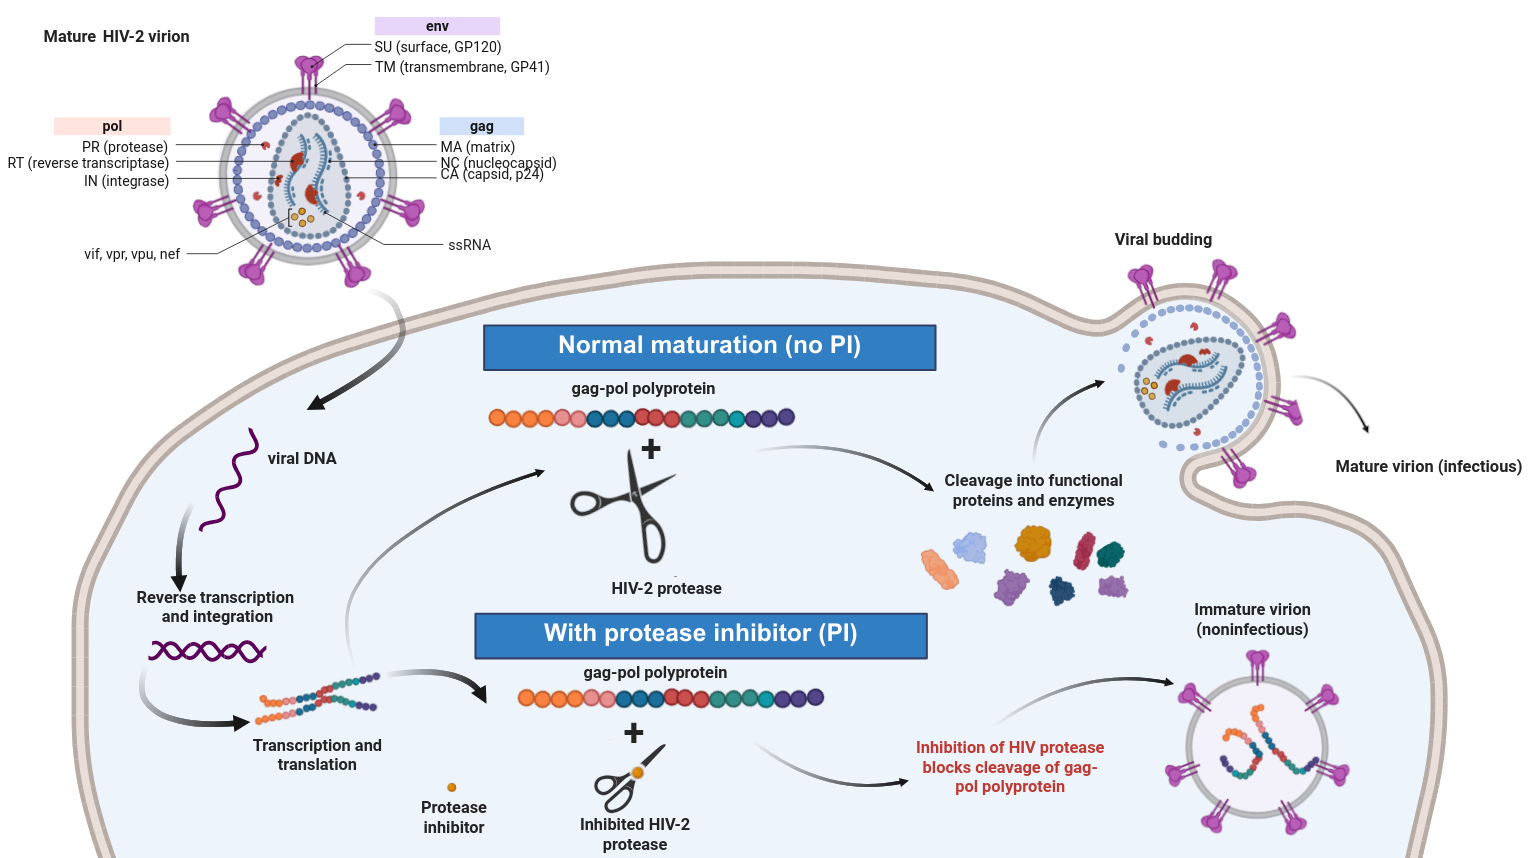
\includegraphics[width=\linewidth]{Figures/Maturation_Inhibition.png}
		\caption{Schéma du rôle de la protéase dans la maturation du VIH2. Inhibiteur de protéase (\textit{protease inhibitor}) empêche les clivages des polyprotéines. Créé en \href{https://www.biorender.com/}{BioRender}, inspiré depuis H.S.Rajput de Pharmacy Freak~\cite{rajput_mechanism_2026}.}
		\label{fig:hiv2_maturation}
	\end{figure}


	\subsection{Protocole de simulations de dynamique moléculaire (DM)} \label{A2}
	Les simulations MD ont été effectuées avec GROMACS 2022 appliqué le champ de force AMBER99SB et mode TIP3P (au moins $1.0$ nm de solvant entre le soluté et bords de boîte). Neutralisation du système a été faite en ajoutant Na et Cl. Pour toutes les simulations, la minimisation était réalisée avec l'algorithme \textit{steepest descent} jusqu'à ce que la force maximale soit réduite en dessous de $1000$ $\text{kJ}\cdot\text{mol}^{-1}\cdot\text{nm}^{-1}$, avec un maximum de $50 000$ étapes de minimisation. L'équilibrage a été effectué en deux étapes : NVT (310 K, thermostat : V-rescale) et NPT (1 bar, barostat : Parrinello-Rahman).\\
	Les interactions électrostatiques à longue portée ont été traitées avec la méthode Particle Mesh Ewald (PME), en utilisant un espacement de grille de Fourier de 0,16 nm et d'interpolation de quatrième ordre. Les interactions Van der Waals et l'électrostatique à courte portée ont été calculés avec une coupure de 1,0 nm, et les interactions non liées ont été gérées à l'aide du schéma de coupure Verlet. Toutes les liaisons covalentes impliquant des atomes d'hydrogène ont été contraintes à l'aide de LINCS, permettant l'utilisation de l'étape de temps de 2 fs tout au long.\\
	L'étape de production, en conditions NPT (310 K, 1 bar) varie en durée pour les simulations : soit 1000 ns, soit 500 ns. Les coordonnées ont été sauvegardées toutes les 10 ps.
	
	\subsection{Formule de RMSD} \label{A3}
	
	\begin{equation}
		{\displaystyle {\begin{aligned}\mathrm {RMSD} (\mathbf {a} ,\mathbf {b} )& ={\sqrt {{\frac {1}{n}}\sum _{i=1}^{n}\|r_{i}(a)-r_{i}(b)\|^{2}}}
					\\ & n= \text{nombre d'atomes}
					\\ & \text{a et b} = \text{2 conformations différentes}
					\\ & r_{i}(a) = \text{vecteur position de l’atome i dans la conformation a}
					\\ & r_{i}(b) = \text{vecteur position de l’atome i dans la conformation b}
		\end{aligned}}}
		\label{eq:RMSD}    
	\end{equation}
	
	\subsection{Formule de RMSF} \label{A4}
	\begin{equation}
		{\displaystyle {\begin{aligned}\mathrm {RMSF}_i & ={\sqrt {{\frac {1}{nsteps}}\sum _{t=1}^{nsteps}\|r_{i}(t)-\langle r_{i}\rangle \|^{2}}}
					\\ & r_{i}(t) = \text{vecteur position de l’atome i au pas t}
					\\ & nsteps = \text{nombre de pas de simulation}
					\\ & \langle r_{i}\rangle = {\frac {1}{nsteps}}\sum _{t=1}^{nsteps} r_i(t) \text{ (positions atomiques moyennes)}
		\end{aligned}}}
		\label{eq:RMSF}    
	\end{equation}

	\subsection{Figures additionnelles, Pt. 2.2.5} \label{A5}
	\begin{figure}[h]
		\centering
		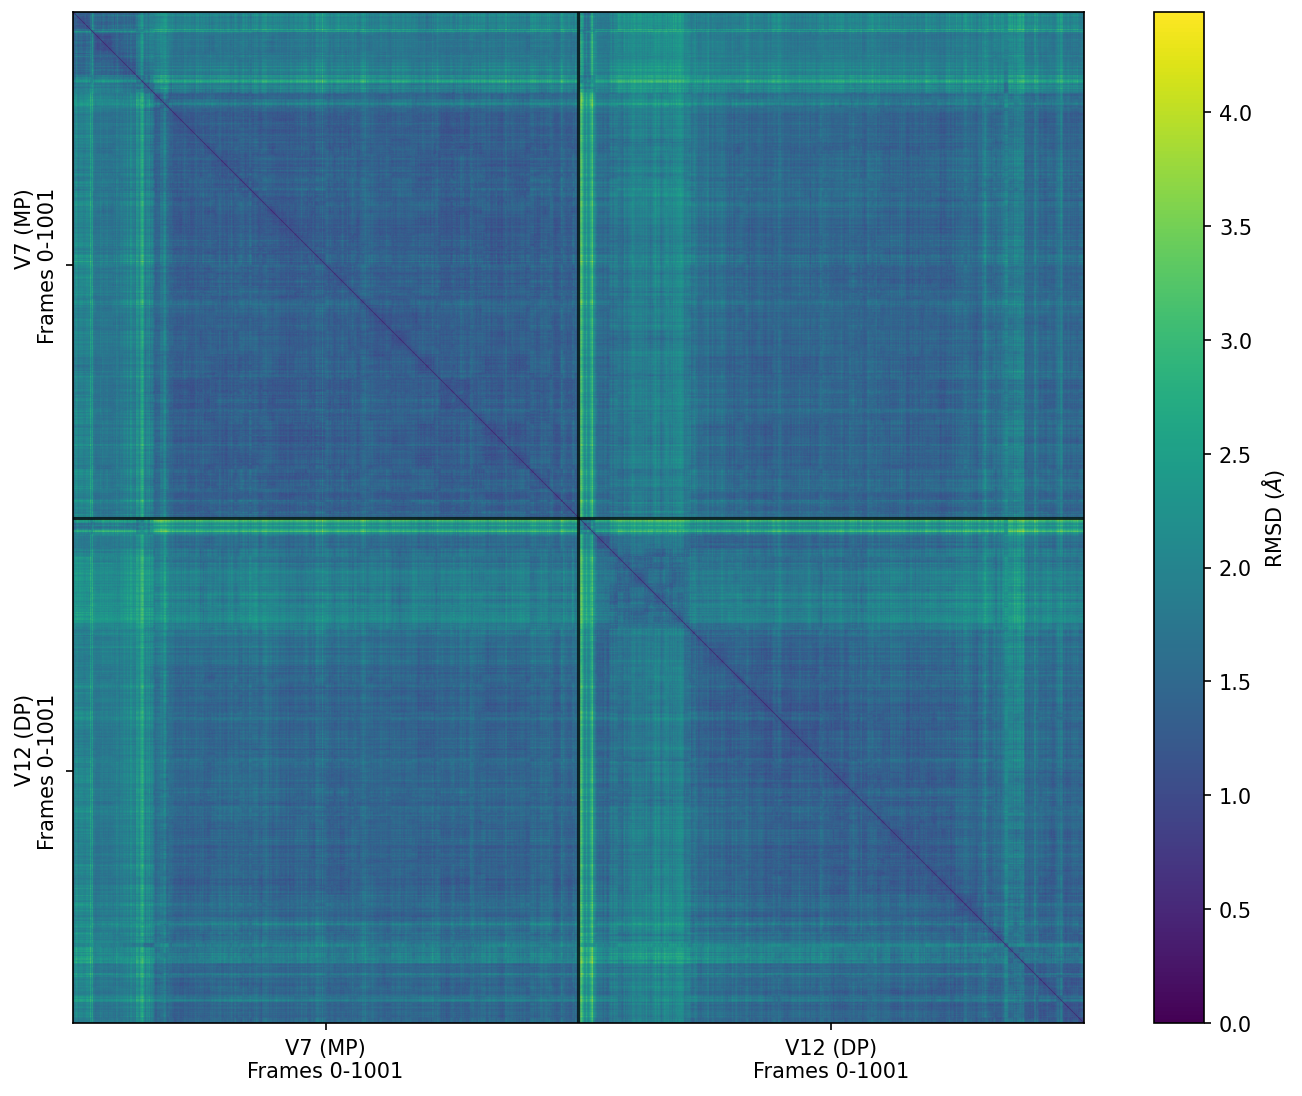
\includegraphics[width=0.7\linewidth]{Figures/pw_rmsd_V7_V12.png}
		\caption{Heatmap représentant la matrice de distances de RMSD par paires pour les deux simulations V7 (MP) et V12 (DP).}
		\label{fig:pw_RMSD}
	\end{figure}
	\newpage
	\subsection{Figures additionnelles, Pt. 3.4} \label{A6}

	\begin{figure}[h]
		\centering
		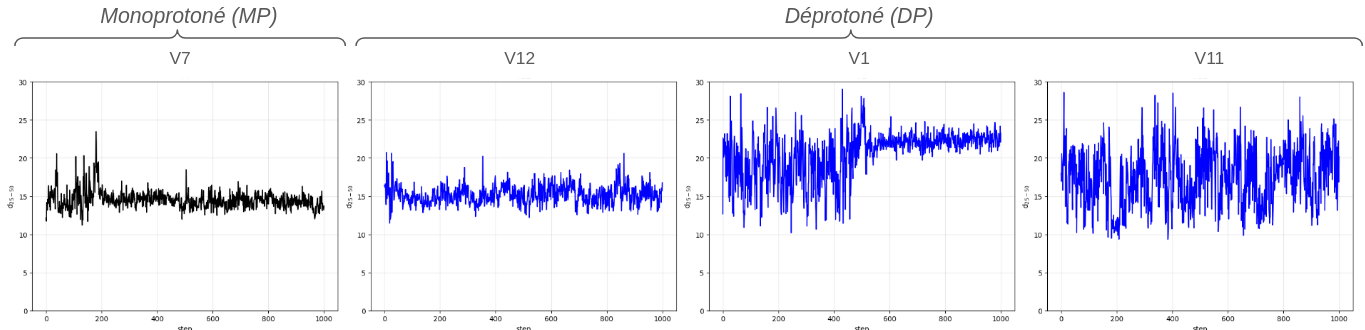
\includegraphics[width=\linewidth]{Figures/d_25_50_chA_new.png}
		\caption{Analyse $d_{25-50}$ la chaine A pour les quatre simulations : DP (V1,V11,V12) en bleu contre référence MP (V7) en noir.}
		\label{fig:d25_50_chA}
	\end{figure}
	
	\begin{figure}[h]
		\centering
		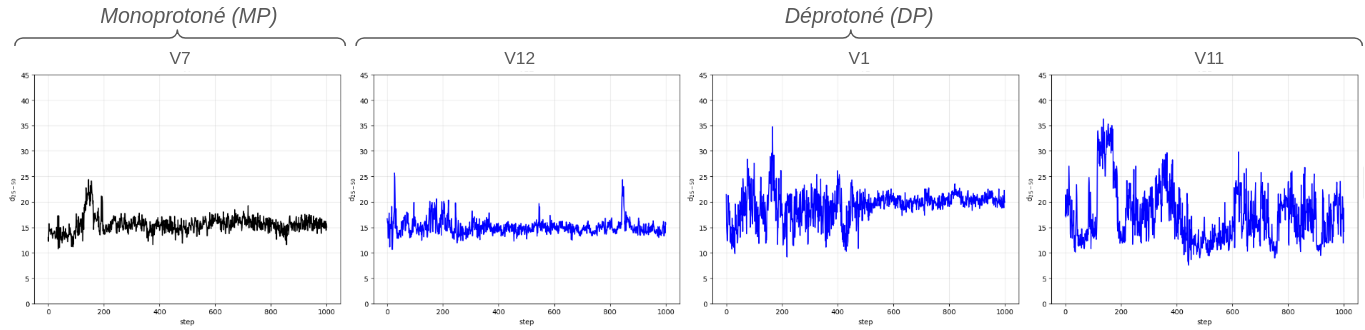
\includegraphics[width=\linewidth]{Figures/d_25_50_chB_new.png}
		\caption{Analyse $d_{25-50}$ la chaine B pour les quatre simulations : DP (V1,V11,V12) en bleu contre référence MP (V7) en noir.}
		\label{fig:d25_50_chB}
	\end{figure}

	\newpage
	\subsection{Figures additionnelles, Pt. 3.5} \label{A7}

	\begin{figure}[h]
		\centering
		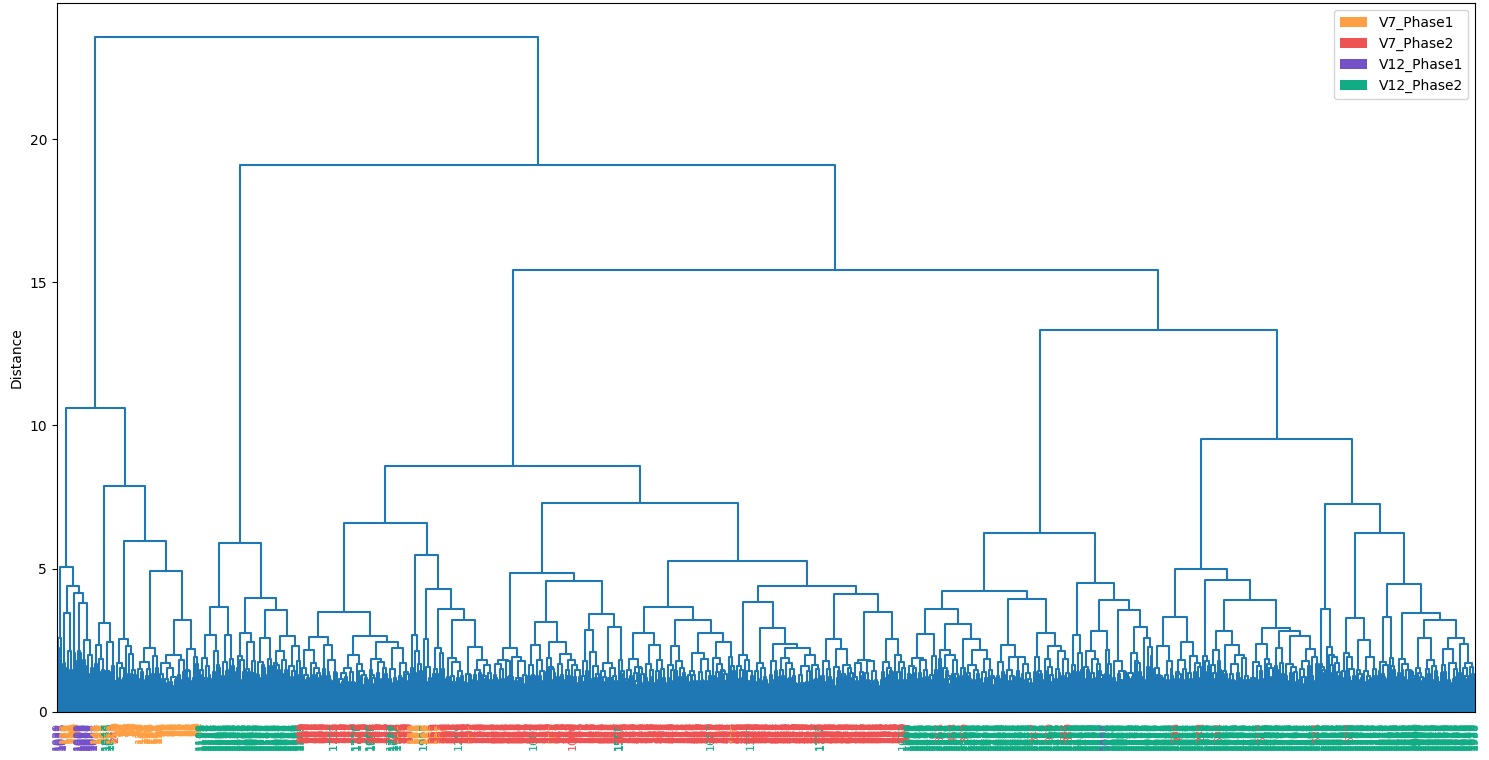
\includegraphics[width=\linewidth]{Figures/dendrogram_jaccard_sim_complete_new.png}
		\caption{Regroupement de frames individuels de V7 (MP) et V12 (DP) basé sur le $\text{RMSD}_{\text{pairs}}$ (méthode Ward).}
		\label{fig:dendro_RMSD}
	\end{figure}

	\begin{figure}[h]
		\centering
		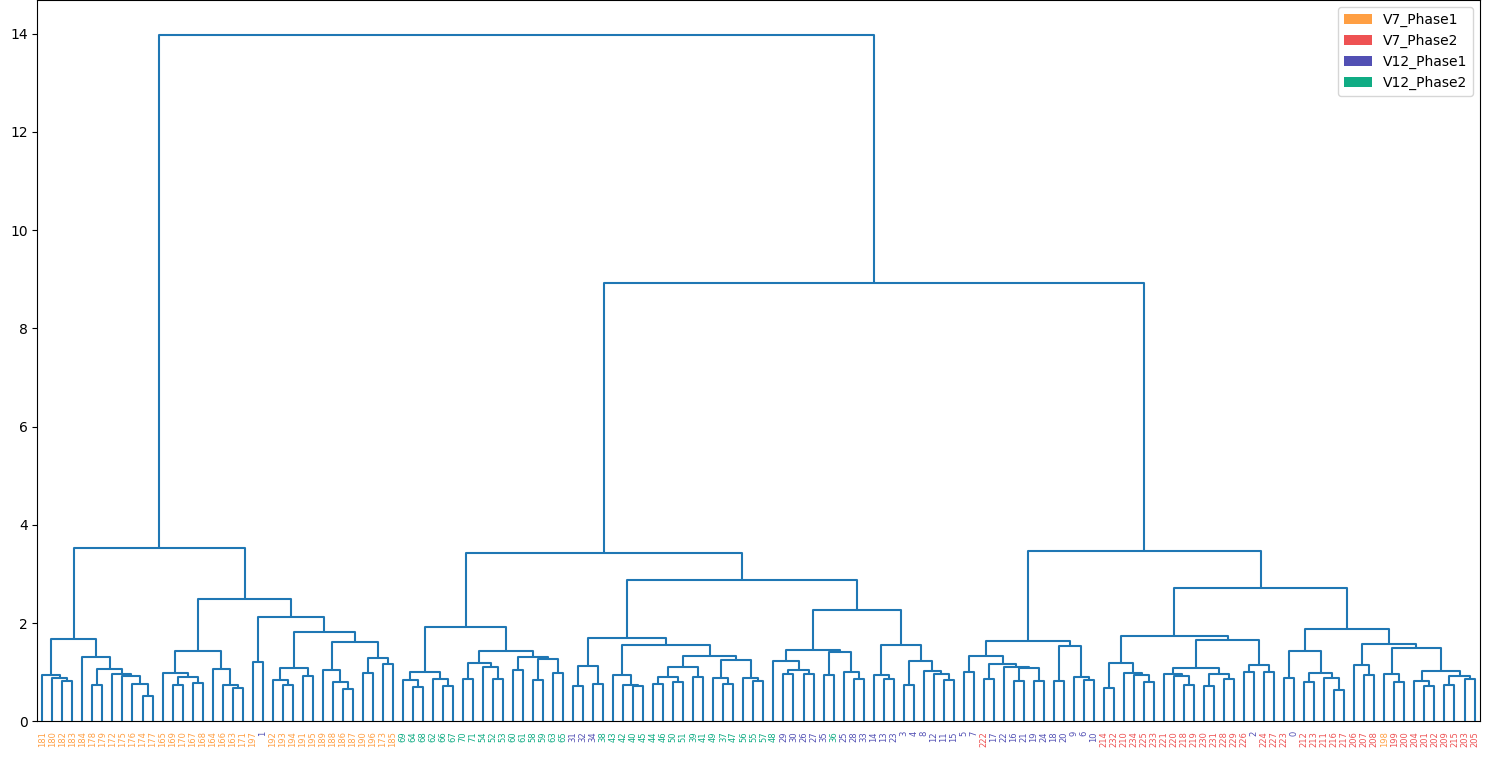
\includegraphics[width=\linewidth]{Figures/dendrogram_jaccard_sim_new.png}
		\caption{Regroupement de frames individuels de V7 (MP) et V12 (DP) au moment de transition entre deux phases ($\pm36~\text{ns}$) basé sur la distance de Jaccard (méthode Ward)}
		\label{fig:dendro_Jaccard}
	\end{figure}

	\cleardoublepage
	
\end{document}